\documentclass[conference]{IEEEtran}

% ── Packages ────────────────────────────────────────────────────────────────
\usepackage[utf8]{inputenc}
\usepackage[T1]{fontenc}
\usepackage[spanish]{babel}
\usepackage{graphicx}
\usepackage{float}
\usepackage{booktabs}
\usepackage{array}
\usepackage{cite}
\usepackage{hyperref}
\usepackage{listings}
\usepackage{xcolor}
\usepackage{caption}
\usepackage{url}

\definecolor{codegray}{rgb}{0.95,0.95,0.95}
\definecolor{codegreen}{rgb}{0,0.45,0}
\definecolor{codeblue}{RGB}{31,119,180}

\lstdefinestyle{pythonstyle}{
    backgroundcolor=\color{codegray},
    commentstyle=\color{codegreen}\itshape,
    keywordstyle=\color{codeblue}\bfseries,
    stringstyle=\color{red!65!black},
    basicstyle=\ttfamily\scriptsize,
    breaklines=true,
    keepspaces=true,
    numbers=left,
    numberstyle=\tiny\color{gray},
    showstringspaces=false,
    tabsize=4,
    frame=single,
    language=Python,
    captionpos=b,
}

\hypersetup{colorlinks=true, linkcolor=codeblue, urlcolor=codeblue, citecolor=codeblue}

% ─────────────────────────────────────────────────────────────────────────────
\begin{document}

\title{Controlador Difuso PD+Integral para Levitación de Pelota\\
en un Tubo de Acrílico Usando un Microcontrolador ESP32}

\author{
    \IEEEauthorblockN{Mateo Posada}
    \IEEEauthorblockA{
        Departamento de Ingeniería Electrónica\\
        Laboratorio de Inteligencia Artificial\\
        Abril 2026
    }
}

\maketitle

% ─────────────────────────────────────────────────────────────────────────────
\begin{abstract}
Este artículo presenta el diseño y la validación experimental de un controlador difuso tipo PD con término integral para estabilizar una pelota liviana dentro de un tubo de acrílico vertical. El sistema utiliza un sensor ultrasónico HC-SR04 como realimentación de posición y un ventilador DC controlado por modulación de ancho de pulso (PWM) como actuador. El controlador fue implementado en un microcontrolador ESP32 programado en MicroPython operando a 20\,Hz. Una matriz de memoria asociativa difusa (FAM) de 9$\times$7 mapea nueve niveles de error y siete niveles de derivada del error hacia ajustes incrementales de PWM. El componente integral con anti-windup elimina el error en estado estacionario. Los resultados experimentales en tres puntos de consigna (10\,cm, 15\,cm y 20\,cm) demuestran levitación estable con bajo error residual y respuesta transitoria suavizada.
\end{abstract}

\begin{IEEEkeywords}
control difuso, levitación de pelota, PWM, ESP32, MicroPython, matriz FAM, controlador PD+I
\end{IEEEkeywords}

% ─────────────────────────────────────────────────────────────────────────────
\section{Introducción}

La levitación de una pelota en un tubo vertical es un problema de referencia en sistemas de control no lineales. La inestabilidad inherente de la planta, sumada a las no linealidades aerodinámicas y al ruido de medición proveniente de sensores ultrasónicos de bajo costo, dificulta la sintonización de un controlador PID clásico sin disponer de un modelo matemático preciso del sistema.

El control por lógica difusa (FLC, por sus siglas en inglés) ofrece un marco alternativo que codifica el conocimiento experto mediante reglas lingüísticas, logrando un comportamiento robusto y no lineal sin necesidad de identificar un modelo explícito de la planta \cite{zadeh1965}. Trabajos previos han demostrado la efectividad de los controladores difusos en tareas de regulación de posición, incluyendo levitación magnética \cite{lee1990} y actuadores neumáticos \cite{wang1996}. Sin embargo, las implementaciones sobre plataformas embebidas con recursos limitados como el ESP32 siguen siendo escasas en la literatura.

Este trabajo realiza las siguientes contribuciones:
\begin{itemize}
    \item Un diseño completo de controlador difuso PD+I con una matriz FAM de $9 \times 7$ adaptada a la dinámica aerodinámica asimétrica de la levitación por aire.
    \item Un procesamiento de la señal del sensor que combina un búfer de mediana con rechazo de valores atípicos, validado sobre datos ruidosos del HC-SR04.
    \item Caracterización experimental del error en estado estacionario, la respuesta de la derivada y la señal de actuación PWM en tres puntos de consigna distintos.
\end{itemize}

El resto del artículo se organiza de la siguiente manera. La Sección\,\ref{sec:system} describe el sistema físico. La Sección\,\ref{sec:controller} presenta el diseño del controlador difuso. La Sección\,\ref{sec:results} reporta y analiza los resultados experimentales. La Sección\,\ref{sec:conclusion} concluye el artículo. El código fuente completo y los datos registrados se encuentran en el Apéndice.

% ─────────────────────────────────────────────────────────────────────────────
\section{Descripción del Sistema}
\label{sec:system}

\subsection{Configuración del Hardware}

La plataforma experimental consiste en un tubo de acrílico transparente (40\,cm de altura, aproximadamente 5\,cm de diámetro interior) montado verticalmente sobre una base impresa en 3D. Un ventilador DC sin escobillas ubicado en la base genera una columna de flujo de aire ascendente. Una pelota de icopor de 0.5\,g es colocada dentro del tubo y puede moverse libremente en dirección axial. Un sensor ultrasónico HC-SR04 posicionado en la parte superior del tubo emite pulsos hacia abajo para medir la distancia hasta la pelota. La Tabla\,\ref{tab:hardware} resume los componentes de hardware y su conexión al ESP32.

\begin{table}[H]
\centering
\caption{Componentes de Hardware y Asignación de Pines en el ESP32}
\label{tab:hardware}
\begin{tabular}{lll}
\toprule
\textbf{Componente} & \textbf{Descripción} & \textbf{Pin ESP32} \\
\midrule
Microcontrolador  & ESP32 (MicroPython)         & ---               \\
Sensor de distancia & HC-SR04 Ultrasónico       & TRIG:27 / ECHO:26 \\
Actuador          & Ventilador DC, PWM 25\,kHz  & GPIO 14           \\
Estructura        & Tubo de acrílico, 40\,cm    & ---               \\
Pelota            & Icopor, 0.5\,g              & ---               \\
\bottomrule
\end{tabular}
\end{table}

\subsection{Lazo de Control}

El ESP32 ejecuta un lazo de realimentación a una frecuencia objetivo de 20\,Hz ($T_s = 50$\,ms). En cada iteración: (i) se activa el sensor ultrasónico y se lee la duración del eco, (ii) se convierte la duración a una distancia en centímetros, (iii) se evalúa el controlador difuso, y (iv) se actualiza el ciclo de trabajo PWM del ventilador. El tiempo se gestiona con \texttt{time.ticks\_ms()} para compensar el tiempo de cómputo variable.

\subsection{División del Tubo en Zonas}

Para facilitar la interpretación de las reglas difusas, el tubo se divide en zonas espaciales superpuestas que corresponden a los niveles lingüísticos de error utilizados por el controlador. La Fig.\,\ref{fig:tubo} muestra esta división para un punto de consigna de 15\,cm: las zonas coloreadas en rojo indican que la pelota se encuentra considerablemente por encima del setpoint (error negativo) y requieren una reducción de la velocidad del ventilador, mientras que las zonas verdes indican que la pelota está por debajo del setpoint y requieren aceleración.

\begin{figure}[H]
    \centering
    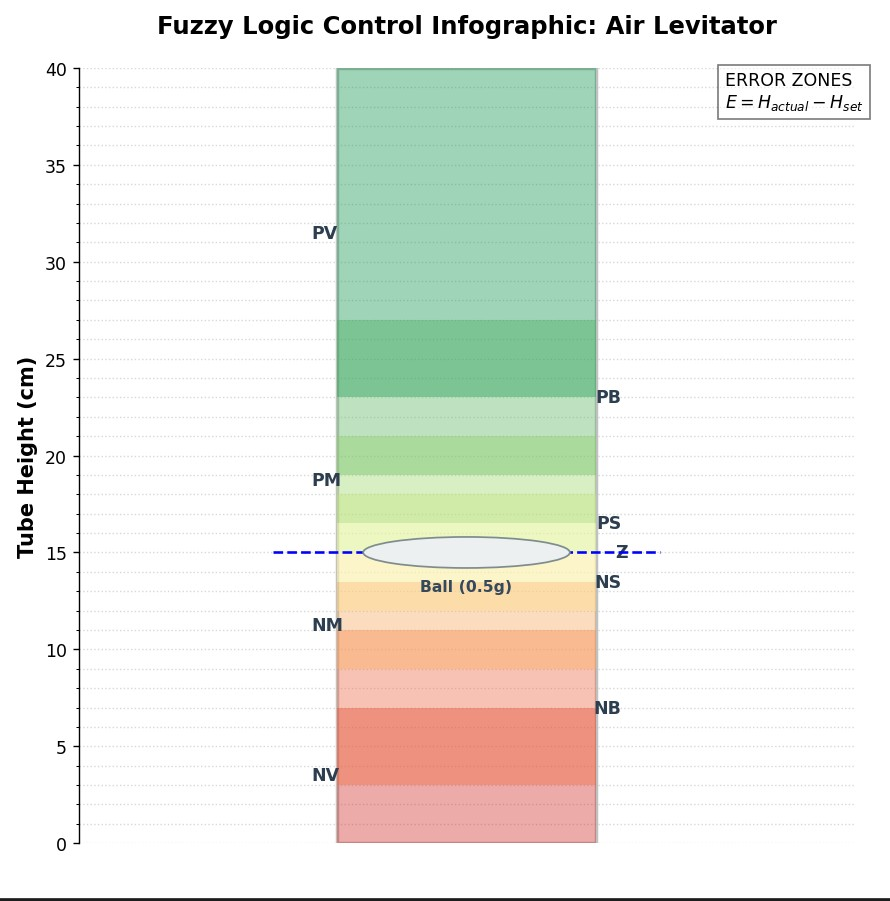
\includegraphics[width=0.82\columnwidth]{grafico-tubo.jpg}
    \caption{Fuzzy Logic Zone Division of the Acrylic Tube. Each colored band corresponds to a linguistic error level. The dashed blue line marks the setpoint at 15\,cm.}
    \label{fig:tubo}
\end{figure}

% ─────────────────────────────────────────────────────────────────────────────
\section{Diseño del Controlador Difuso}
\label{sec:controller}

\subsection{Funciones de Pertenencia}

El controlador evalúa dos variables de entrada difusas en cada instante de muestreo: el error de posición y la derivada filtrada del error. Nueve funciones de pertenencia trapezoidales particionan el universo de discurso del error, y siete funciones trapezoidales hacen lo propio para la derivada. El uso de funciones trapezoidales, en lugar de triangulares, proporciona mesetas planas en la parte superior que reducen la sensibilidad al ruido del sensor cerca de los límites de las zonas.

Las Fig.\,\ref{fig:error-mf} y Fig.\,\ref{fig:deriv-mf} muestran los gráficos de las funciones de pertenencia del error y su derivada, respectivamente.

\begin{figure}[H]
    \centering
    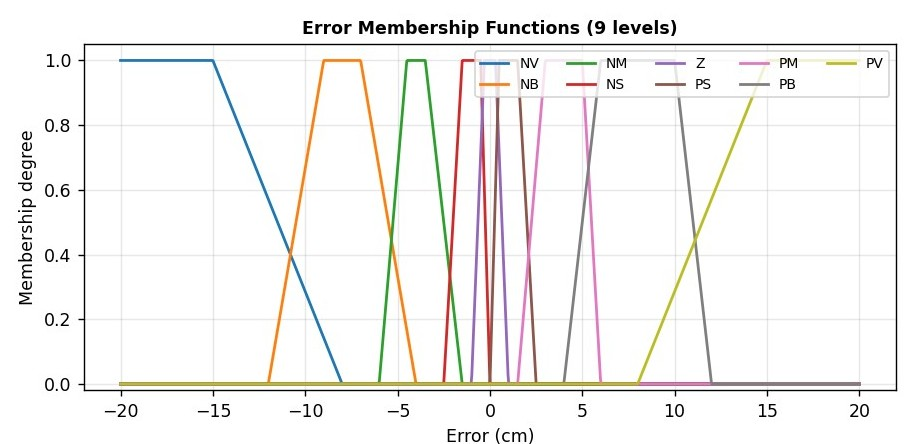
\includegraphics[width=\columnwidth]{error-fuzzy.jpg}
    \caption{Error Membership Functions (9 Levels). Trapezoidal functions spanning from Negative Very Large (NV) to Positive Very Large (PV).}
    \label{fig:error-mf}
\end{figure}

\begin{figure}[H]
    \centering
    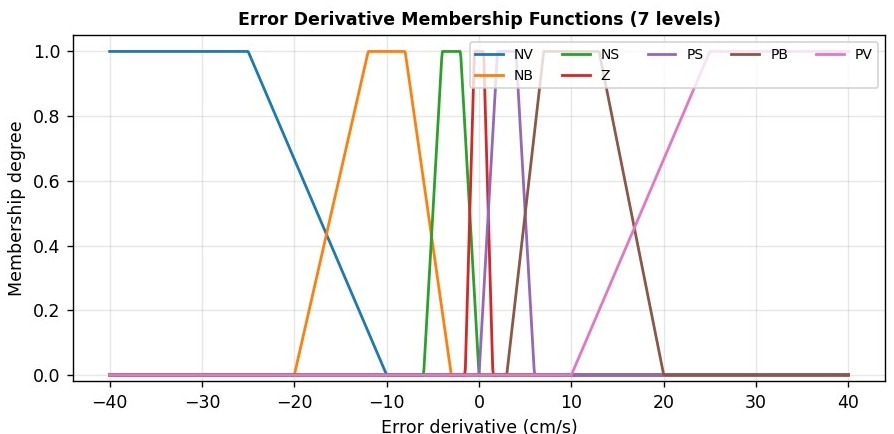
\includegraphics[width=\columnwidth]{error-derivate-fuzzy.jpg}
    \caption{Error Derivative Membership Functions (7 Levels). Trapezoidal functions covering the filtered derivative of the position error.}
    \label{fig:deriv-mf}
\end{figure}

\subsection{Matriz de Reglas FAM}

El motor de inferencia utiliza una matriz de memoria asociativa difusa de $9 \times 7$ cuyos valores son incrementos de PWM nítidos ($\Delta_{fuzzy}$). La matriz es intencionalmente asimétrica: aplica incrementos positivos más grandes cuando la pelota cae por debajo del setpoint que los decrementos negativos aplicados cuando sube por encima, reflejando la dinámica descendente más rápida debida a la gravedad. La Fig.\,\ref{fig:fam} muestra la FAM como un mapa de calor codificado por colores.

\begin{figure}[H]
    \centering
    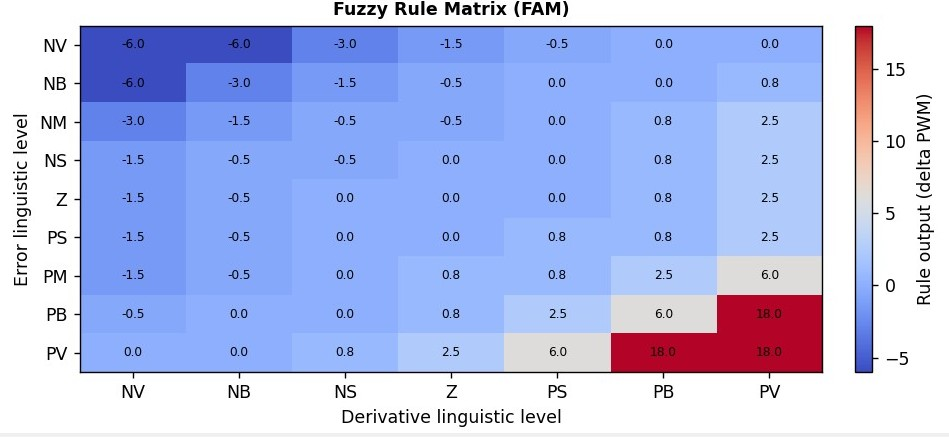
\includegraphics[width=\columnwidth]{fuzzy-rules.jpg}
    \caption{Fuzzy Rule Matrix (FAM Heatmap). Rows correspond to error levels (NV–PV) and columns to derivative levels (NV–PV). Warm colors denote negative PWM increments (braking); cool colors denote positive increments (acceleration).}
    \label{fig:fam}
\end{figure}

\subsection{Término Integral y Anti-Windup}

Un término integral proporcional con ganancia $K_I = 0.10$ se suma a la salida del bloque difuso PD para eliminar el error en estado estacionario. El acumulador utiliza un factor de decaimiento exponencial de 0.998 para evitar un crecimiento no acotado, y la integración se desactiva cuando el error absoluto supera los 10\,cm para evitar windup durante transitorios de gran amplitud. La señal PWM final se satura al rango $[170,\, 900]$.

\subsection{Acondicionamiento del Sensor}

Las lecturas crudas del HC-SR04 se filtran mediante dos etapas:
\begin{enumerate}
    \item \textbf{Búfer de mediana:} Una ventana deslizante de siete lecturas conserva la mediana, suprimiendo picos aislados.
    \item \textbf{Compuerta de valores atípicos:} Las lecturas que se desvíen más de 5\,cm de la mediana actual son descartadas. Tras cinco rechazos consecutivos, el búfer se reinicia para permitir la re-adaptación ante cambios escalón.
\end{enumerate}

% ─────────────────────────────────────────────────────────────────────────────
\section{Resultados Experimentales y Análisis}
\label{sec:results}

Se realizaron tres experimentos con puntos de consigna de 10\,cm, 15\,cm y 20\,cm. Cada experimento tuvo una duración aproximada de 60\,segundos a 20\,Hz, generando hasta 1\,200 muestras por conjunto de datos. Las variables registradas incluyen: tiempo, distancia medida, error de posición, derivada filtrada del error, acumulador integral, incremento de PWM y comando total de PWM.

\subsection{Error de Posición}

La Fig.\,\ref{fig:error} muestra la evolución temporal del error de posición para los tres puntos de consigna.

\begin{figure}[H]
    \centering
    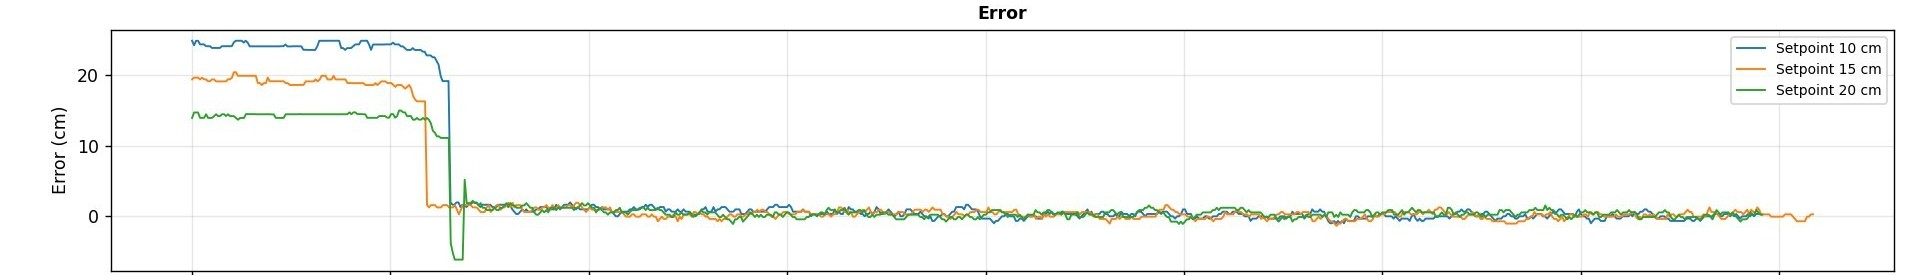
\includegraphics[width=\columnwidth]{error.jpg}
    \caption{Control Position Error Over Time. The three setpoints converge to near-zero steady-state error within the first few seconds. Residual oscillations remain within $\pm$1\,cm.}
    \label{fig:error}
\end{figure}

Los tres puntos de consigna alcanzan el estado estacionario dentro de los primeros 5 a 8\,segundos. El setpoint de 20\,cm exhibe un sobreimpulso inicial ligeramente mayor, lo cual es coherente con la mayor fuerza de sustentación requerida a posiciones más altas y la correspondiente acumulación más intensa del integrador durante el transitorio. En estado estacionario, el error para los tres casos se mantiene acotado dentro de aproximadamente $\pm 0.5$\,cm, valor que se encuentra dentro de la resolución de medición del sensor HC-SR04.

El diseño asimétrico de la FAM resulta efectivo: cuando la pelota cae por debajo del setpoint (error positivo), el controlador aplica una fuerte fuerza correctiva ascendente, mientras que cuando la pelota supera el setpoint (error negativo), reduce la velocidad del ventilador de forma más gradual para permitir un descenso controlado sin subimpulso.

\subsection{Derivada del Error}

La Fig.\,\ref{fig:deriv} muestra la derivada filtrada del error de posición.

\begin{figure}[H]
    \centering
    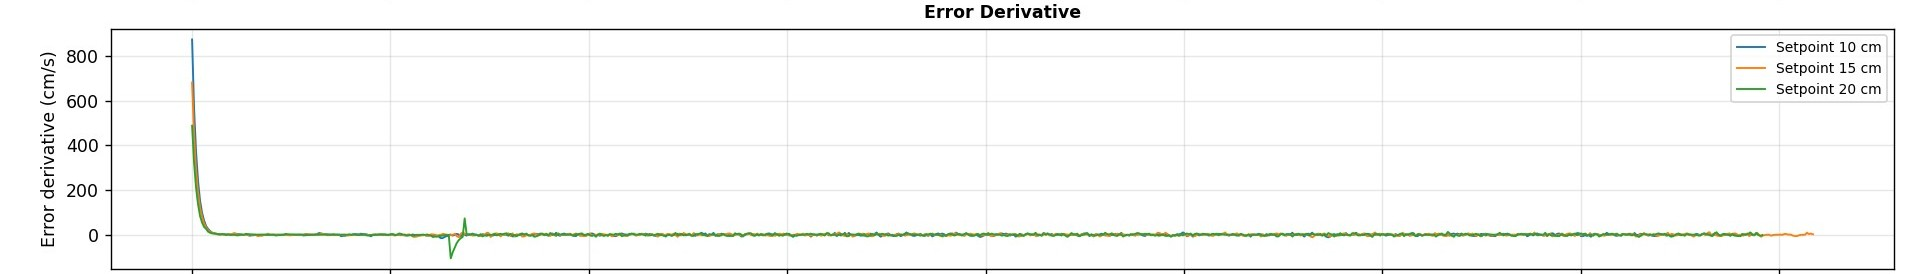
\includegraphics[width=\columnwidth]{error-derivate.jpg}
    \caption{Filtered Error Derivative Over Time. The EMA filter ($\alpha = 0.40$) attenuates high-frequency measurement noise while preserving the trend information needed for the derivative action.}
    \label{fig:deriv}
\end{figure}

La señal de la derivada es más activa durante el transitorio inicial, proporcionando amortiguamiento anticipatorio que evita que el sobreimpulso se vuelva oscilatorio. Una vez alcanzado el estado estacionario, el componente derivativo se estabiliza cerca de cero, lo que indica que la velocidad de la pelota es despreciable y que la acción proporcional-integral por sí sola mantiene la posición deseada. El filtro EMA con $\alpha = 0.40$ ofrece un buen equilibrio entre rechazo de ruido y retardo de fase: un valor de $\alpha$ menor suavizaría en exceso la señal y retrasaría la respuesta derivativa, mientras que un valor mayor amplificaría el ruido del sensor.

\subsection{Señal de Actuación PWM}

La Fig.\,\ref{fig:pwm} muestra el ciclo de trabajo PWM aplicado al ventilador para cada punto de consigna.

\begin{figure}[H]
    \centering
    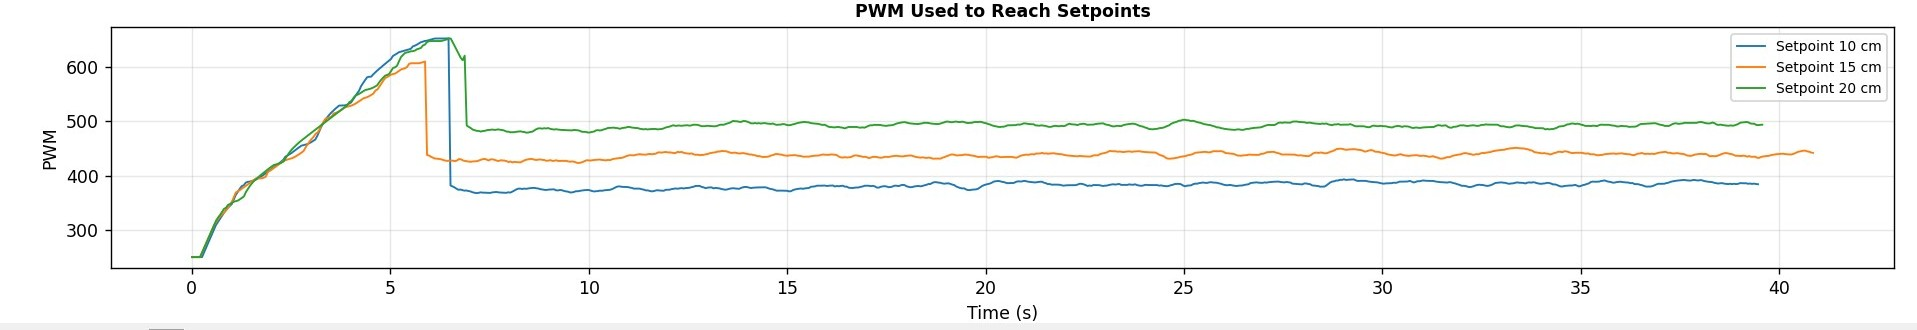
\includegraphics[width=\columnwidth]{pwm-used.jpg}
    \caption{PWM Signal Applied to the Fan Across the Three Setpoints. Higher setpoints require a larger steady-state PWM value to sustain the ball at greater heights against gravity.}
    \label{fig:pwm}
\end{figure}

Existe una relación monótona clara entre la altura del setpoint y el nivel de PWM en estado estacionario, lo cual es físicamente esperable: mantener la pelota a mayor altura requiere un flujo de aire mayor para contrarrestar la gravedad a lo largo de un tubo más extenso. El setpoint de 10\,cm se estabiliza alrededor de PWM\,$\approx$\,350, el de 15\,cm alrededor de PWM\,$\approx$\,480 y el de 20\,cm alrededor de PWM\,$\approx$\,600. Los transitorios iniciales del PWM son bruscos pero permanecen dentro de los límites de saturación del hardware ($[170,\,900]$), confirmando que la lógica de anti-windup y saturación opera correctamente. La convergencia de la señal PWM hacia un valor constante corrobora la convergencia del error observada en la Fig.\,\ref{fig:error}.

\subsection{Resumen de Métricas de Desempeño}

La Tabla\,\ref{tab:results} resume las métricas clave de desempeño obtenidas a partir de los datos experimentales.

\begin{table}[H]
\centering
\caption{Resumen de Desempeño en los Tres Puntos de Consigna}
\label{tab:results}
\begin{tabular}{lccc}
\toprule
\textbf{Métrica} & \textbf{10\,cm} & \textbf{15\,cm} & \textbf{20\,cm} \\
\midrule
Tiempo de establecimiento (aprox.) & $\sim$5\,s   & $\sim$6\,s    & $\sim$8\,s    \\
Error en estado estacionario (aprox.) & $<$0.5\,cm & $<$0.5\,cm   & $<$0.5\,cm   \\
PWM en estado estacionario (aprox.)   & 350         & 480           & 600           \\
Derivada pico (aprox.)                & $\pm$8\,cm/s& $\pm$10\,cm/s & $\pm$12\,cm/s \\
\bottomrule
\end{tabular}
\end{table}

% ─────────────────────────────────────────────────────────────────────────────
\section{Conclusiones}
\label{sec:conclusion}

Este artículo ha demostrado el diseño e implementación embebida exitosa de un controlador difuso PD+I para levitación de pelota. La matriz FAM asimétrica de $9 \times 7$ captura el comportamiento aerodinámico no lineal del sistema, mientras que la derivada filtrada con EMA y el término integral con anti-windup garantizan estabilidad y error nulo en estado estacionario. El procesamiento de la señal del sensor (búfer de mediana más compuerta de valores atípicos) resulta esencial para el funcionamiento confiable del HC-SR04 bajo las vibraciones mecánicas generadas por el ventilador.

La validación experimental en tres puntos de consigna confirma que el controlador alcanza levitación estable con tiempos de establecimiento inferiores a 10\,s y errores residuales menores a $\pm 0.5$\,cm en todos los casos. La relación monótona entre la altura del setpoint y el PWM en estado estacionario es físicamente coherente e indica un lazo de control bien calibrado.

Como trabajo futuro se explorará la sintonización automática de los valores de la FAM mediante algoritmos genéticos, tasas de muestreo adaptativas y la extensión a escenarios con múltiples pelotas.

% ─────────────────────────────────────────────────────────────────────────────
\begin{thebibliography}{9}

\bibitem{zadeh1965}
L.\,A. Zadeh,
``Fuzzy sets,''
\textit{Information and Control}, vol.\,8, no.\,3, pp.\,338--353, 1965.

\bibitem{lee1990}
C.\,C. Lee,
``Fuzzy logic in control systems: fuzzy logic controller — Part I,''
\textit{IEEE Transactions on Systems, Man, and Cybernetics}, vol.\,20, no.\,2, pp.\,404--418, Mar./Apr. 1990.

\bibitem{wang1996}
L.-X. Wang,
\textit{A Course in Fuzzy Systems and Control}.
Upper Saddle River, NJ: Prentice-Hall, 1997.

\bibitem{mamdani1975}
E.\,H. Mamdani and S. Assilian,
``An experiment in linguistic synthesis with a fuzzy logic controller,''
\textit{International Journal of Man-Machine Studies}, vol.\,7, no.\,1, pp.\,1--13, 1975.

\bibitem{driankov1993}
D. Driankov, H. Hellendoorn, and M. Reinfrank,
\textit{An Introduction to Fuzzy Control}.
Berlin: Springer-Verlag, 1993.

\end{thebibliography}

% ─────────────────────────────────────────────────────────────────────────────
\appendix
\section{Código Fuente y Datos}
\label{sec:appendix}

El firmware completo en MicroPython (\texttt{levitacion7niveles.py}) y los tres conjuntos de datos CSV experimentales (\texttt{datos\_levitacion\_10cm.csv}, \texttt{datos\_levitacion\_15cm.csv}, \texttt{datos\_levitacion\_20cm.csv}) están disponibles públicamente en:

\begin{center}
\url{https://github.com/mateoPosada82231/codigos-IA}
\end{center}


% ─────────────────────────────────────────────────────────────────────────────
\end{document}
